\section{Inelastic scattering}

\subsection{General features of inelastic scattering}

\slide{}
\begin{center}
\psframebox[fillcolor=green!10,linecolor=blue,framearc=0.1,fillstyle=solid,framesep=5pt]{
Inelastic scattering
}%psframe
\end{center} 
\end{frame}

% --------------------------------------------------------------------------------------
\slide{Inelastic scattering}
\begin{itemize}
\item Nuclei are not inert or {\em frozen} objects; they do have an internal structure of protons and neutrons
that can be modified (excited) during the collision.
\item Quantum systems exhibit, in general, an energy spectrum with bound and unbound levels.
\end{itemize}

\begin{columns}
\column{0.5\textwidth}
\begin{figure}{\par \resizebox*{0.75\textwidth}{!}
{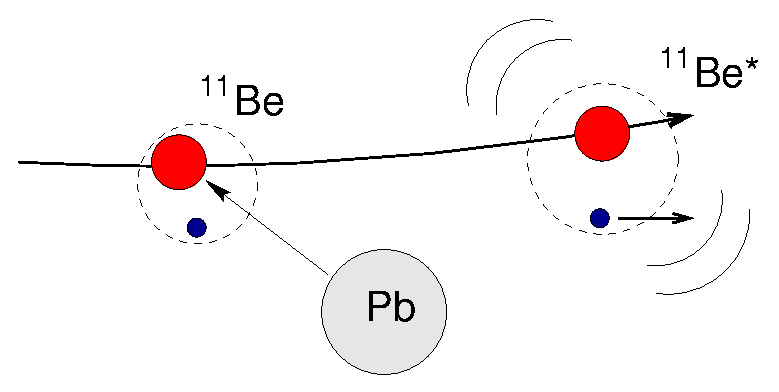
\includegraphics[angle=0]{\images/be11pb_inel.eps}} \par}
\end{figure}
\column{0.5\textwidth}
\begin{figure}{\par \resizebox*{0.5\textwidth}{!}
{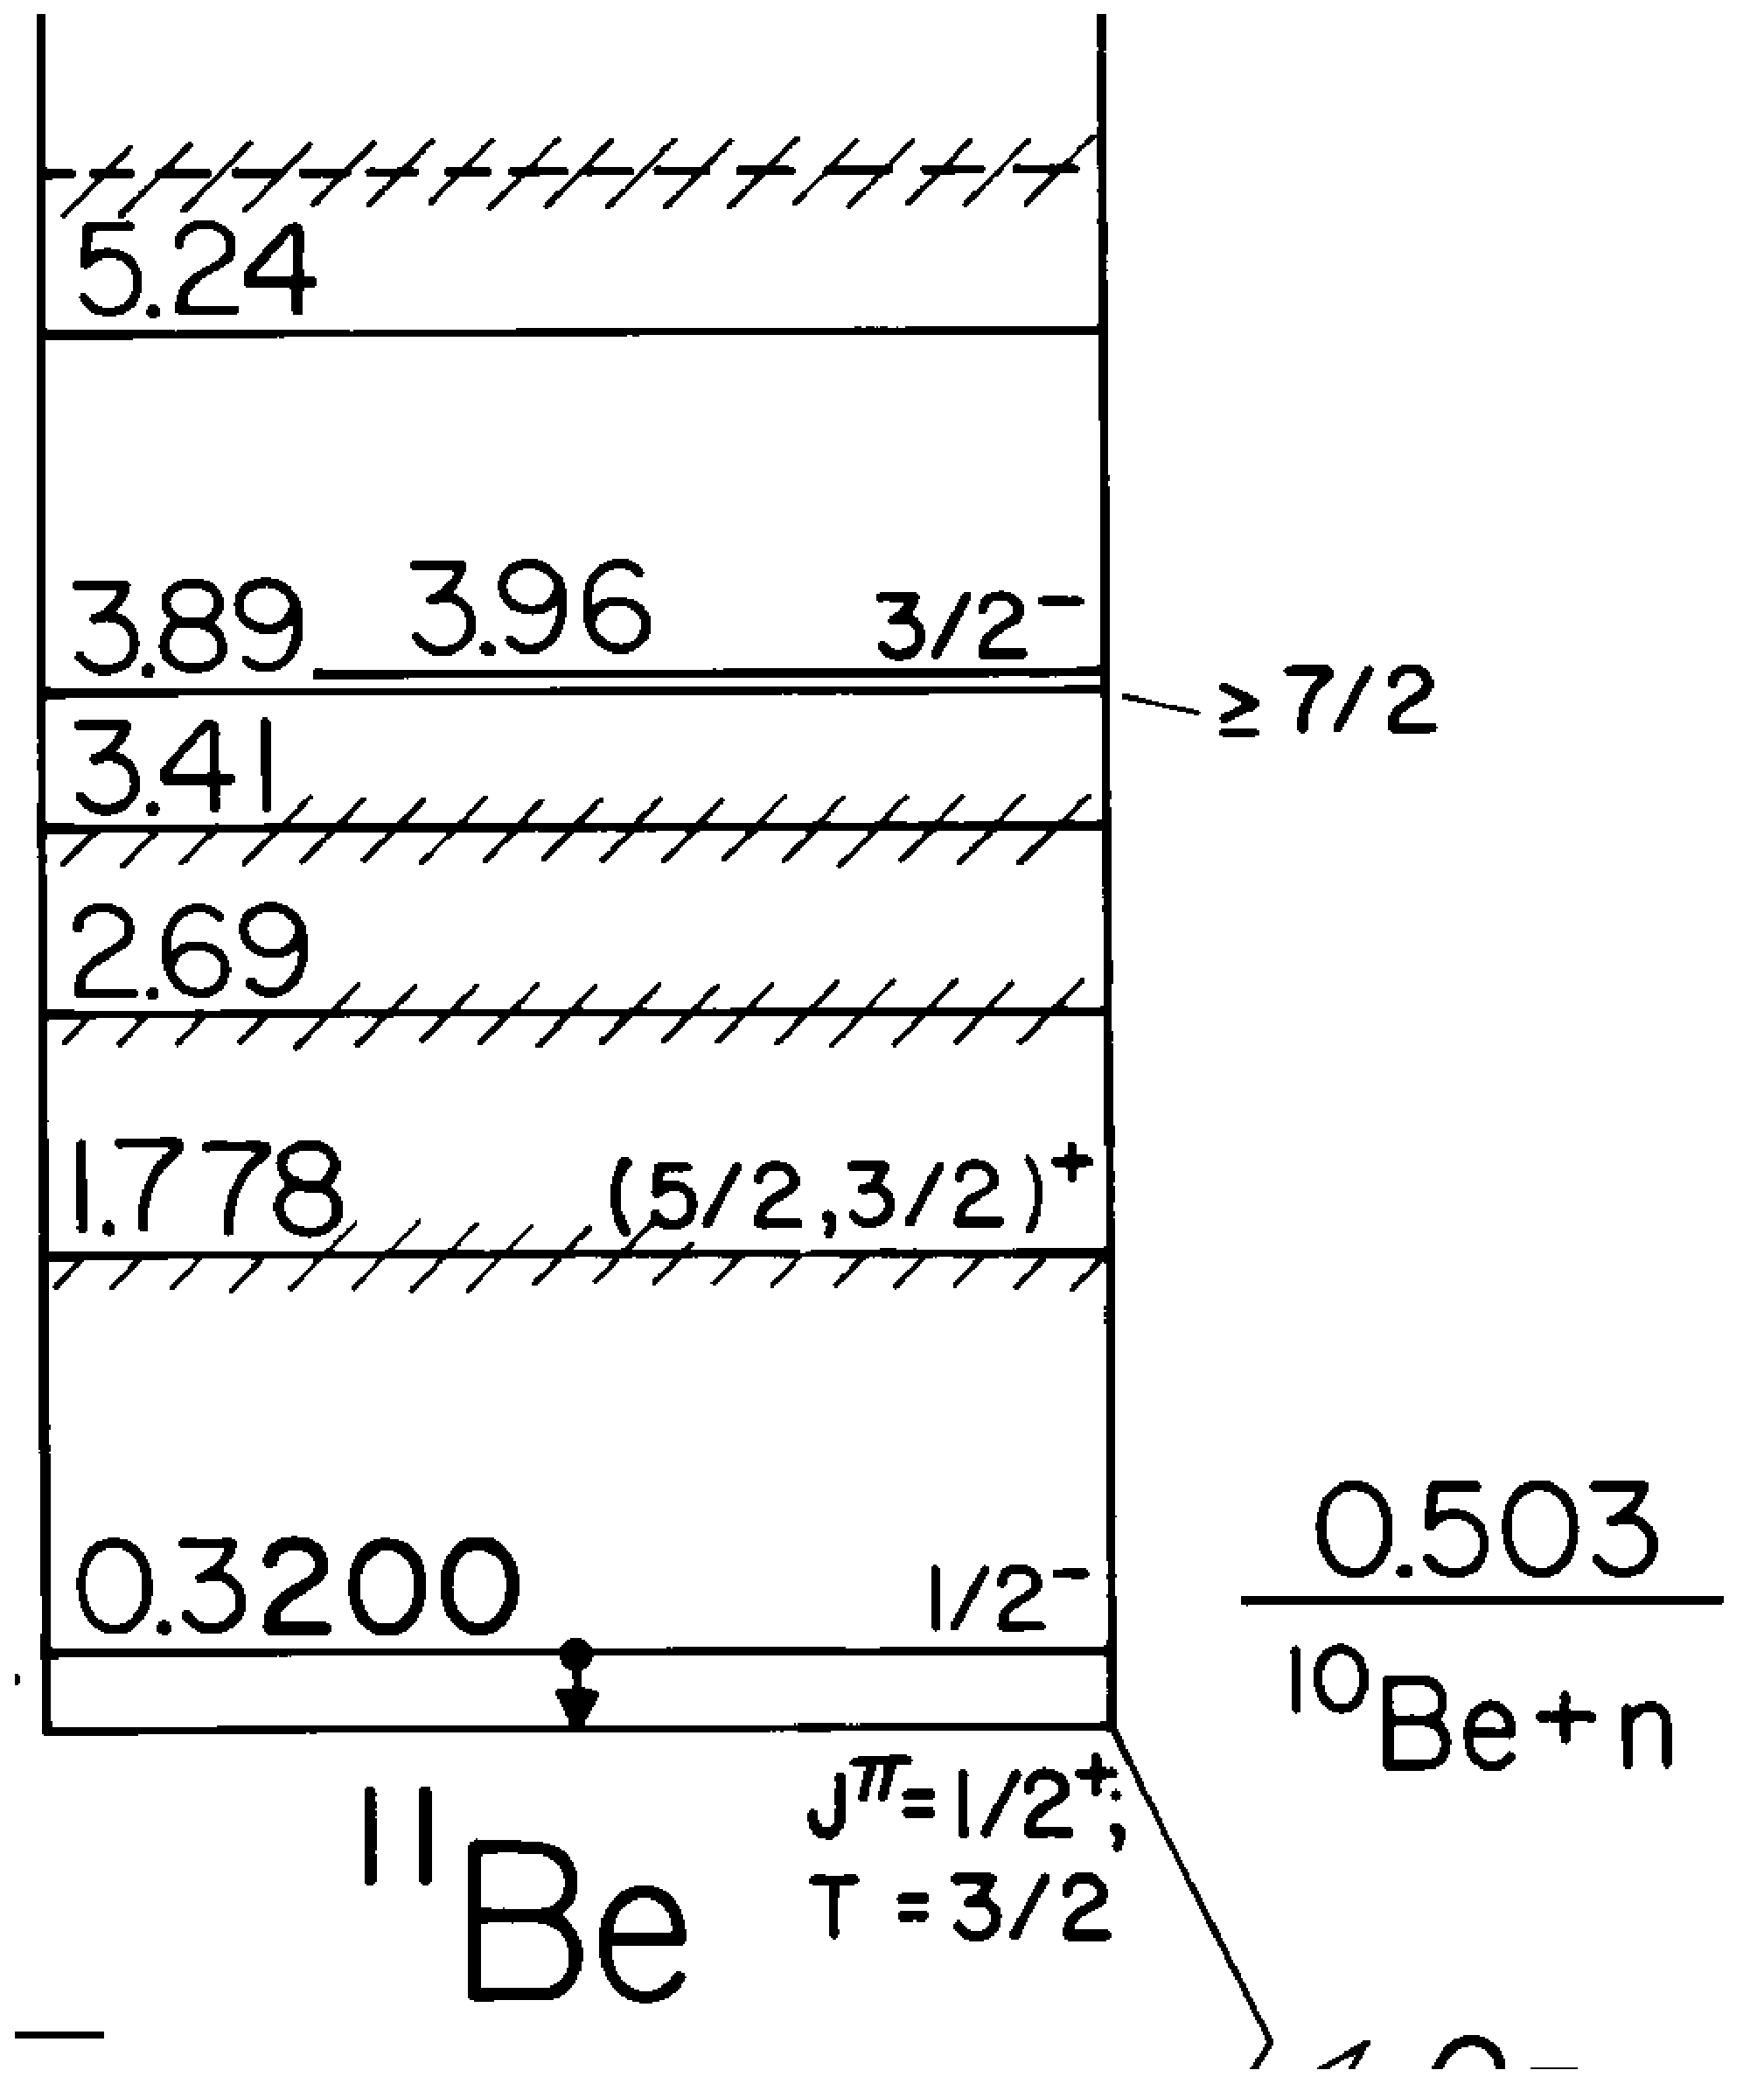
\includegraphics[angle=0]{\images/be11_spectrum_crop.eps}} \par}
\end{figure}
\end{columns}
\end{frame}


%----------------------------------------------------------------------------------------
\slide{Models for inelastic excitations}

\begin{enumerate}
\ritem{\sc COLLECTIVE:} Involve a collective motion of several nucleons which can be interpreted macroscopically as {\verde rotations} or  {\verde surface vibrations} of the nucleus.
 \begin{figure}{\par \resizebox*{0.15\textwidth}{!}
{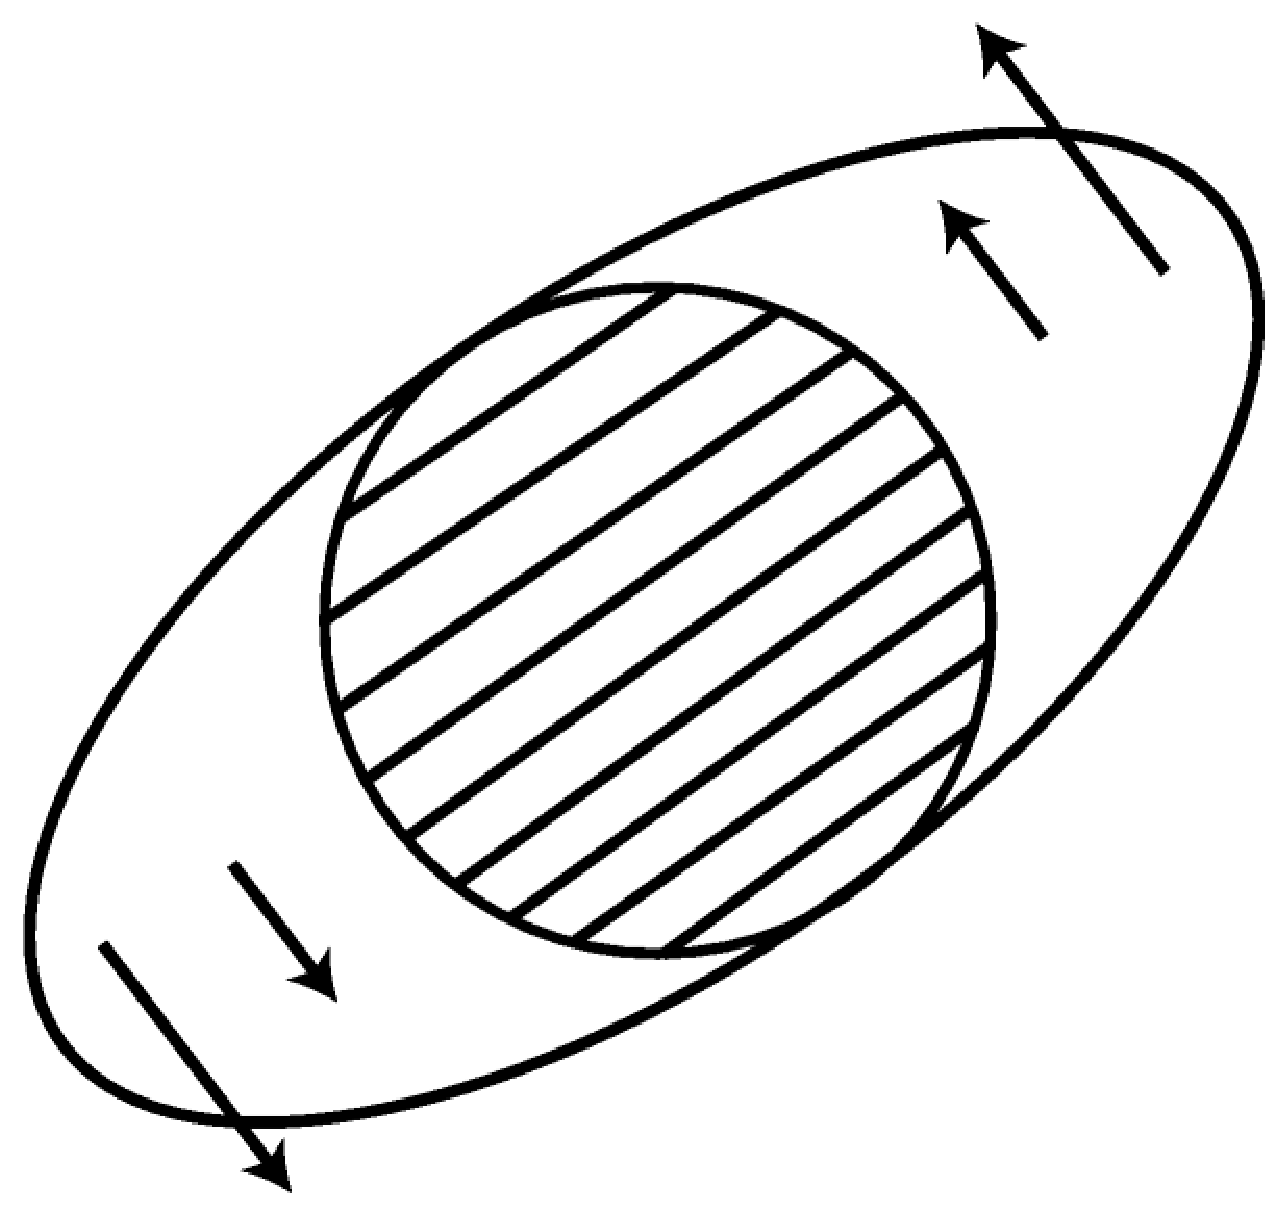
\includegraphics{\images/deformed-nucleus.eps}} \par}
\end{figure}

\ritem{\sc FEW-BODY/SIGLE-PARTICLE:} Involve the excitation of a nucleon or cluster.
\begin{figure}{\par \resizebox*{0.3\textwidth}{!}
{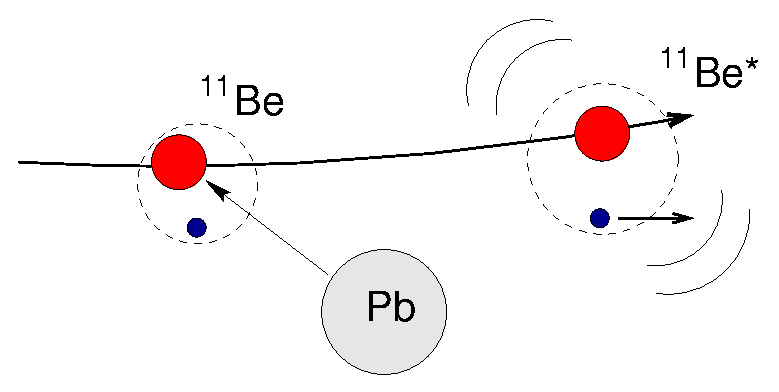
\includegraphics[angle=0]{\images/be11pb_inel.eps}} \par}
\end{figure}
\end{enumerate}

\end{frame}


% ----------------------------------------------------------------------------------
\slide{Types of collective excitations}

\only<1>{
The nucleons can move inside the nucleus in a coherent (collective) way.

\begin{enumerate}
\gitem{Vibrations} (spherical nuclei): small surface oscillations in shape.
\begin{figure}{\par \resizebox*{0.25\textwidth}{!}
{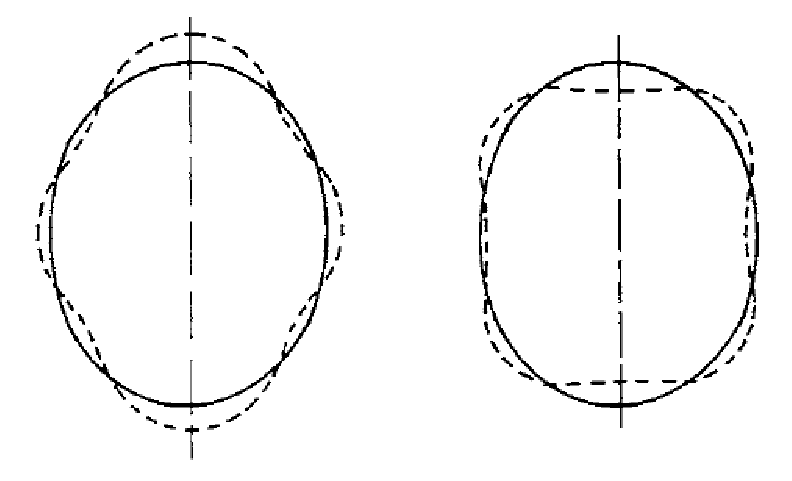
\includegraphics{\images/vibrations.eps}} \par}
\end{figure}
\gitem{Rotations} (non-spherical nuclei): permanent deformation.
\gitem{Monopole} ({\em breathing}) mode: oscillations in the size (radius). 
\gitem{Isovector} excitations (protons and neutrons move out of phase) (eg. giant dipole resonance)
\end{enumerate}
}
\only<2>{
\ding{43} The type of collective motion is closely related to the kind of energy spectrum.
\begin{itemize} 
\item Rotor: $E_J \propto J(J+1)$
\item Vibrator: $E_J \approx n \hbar \omega$
\end{itemize}

\begin{figure}{\par \resizebox*{0.7\textwidth}{!}
%{\includegraphics{\images/vibrational-rotational-spectrum.eps}} \par}
{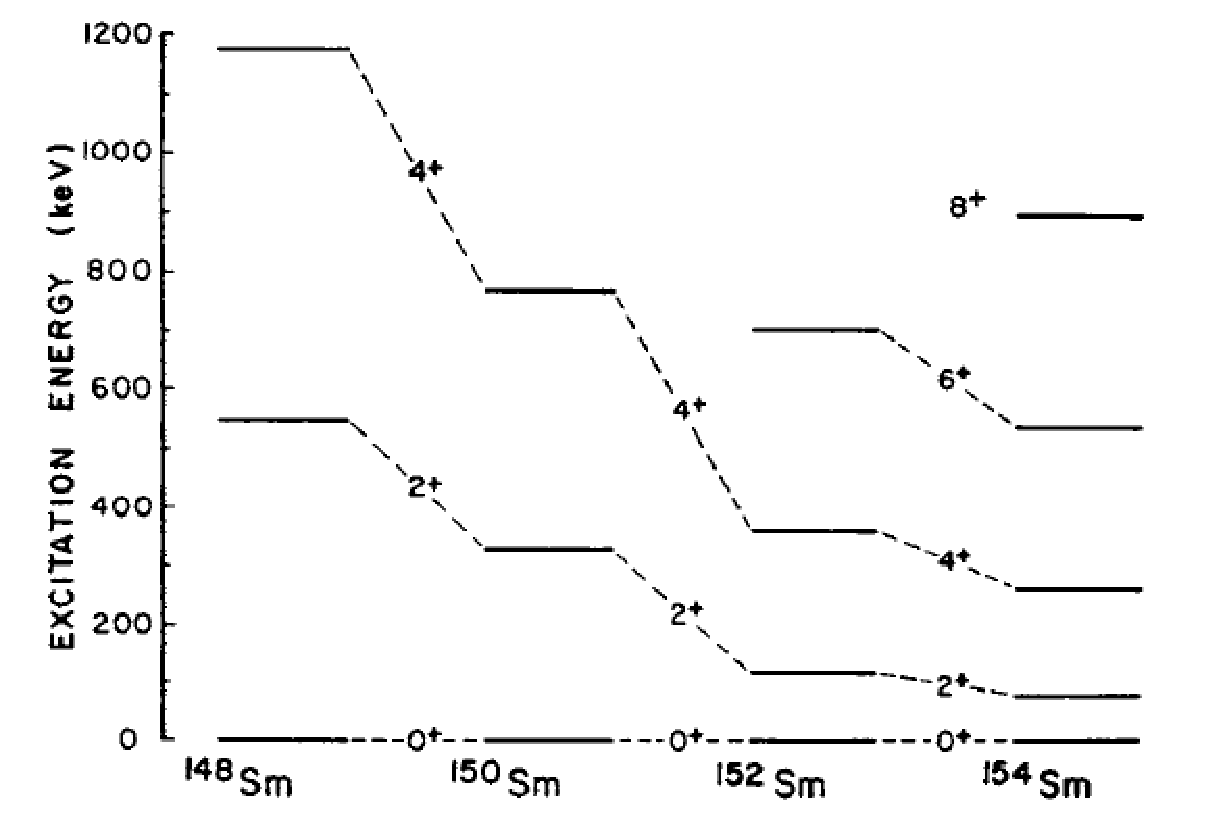
\includegraphics{\images/samarium.eps}} \par}
\end{figure}
}%onslide
\end{frame}



%------------------------------------------------------------
\slide{Microscopic description in the IPM: the $^{11}$Be case} 

\begin{center}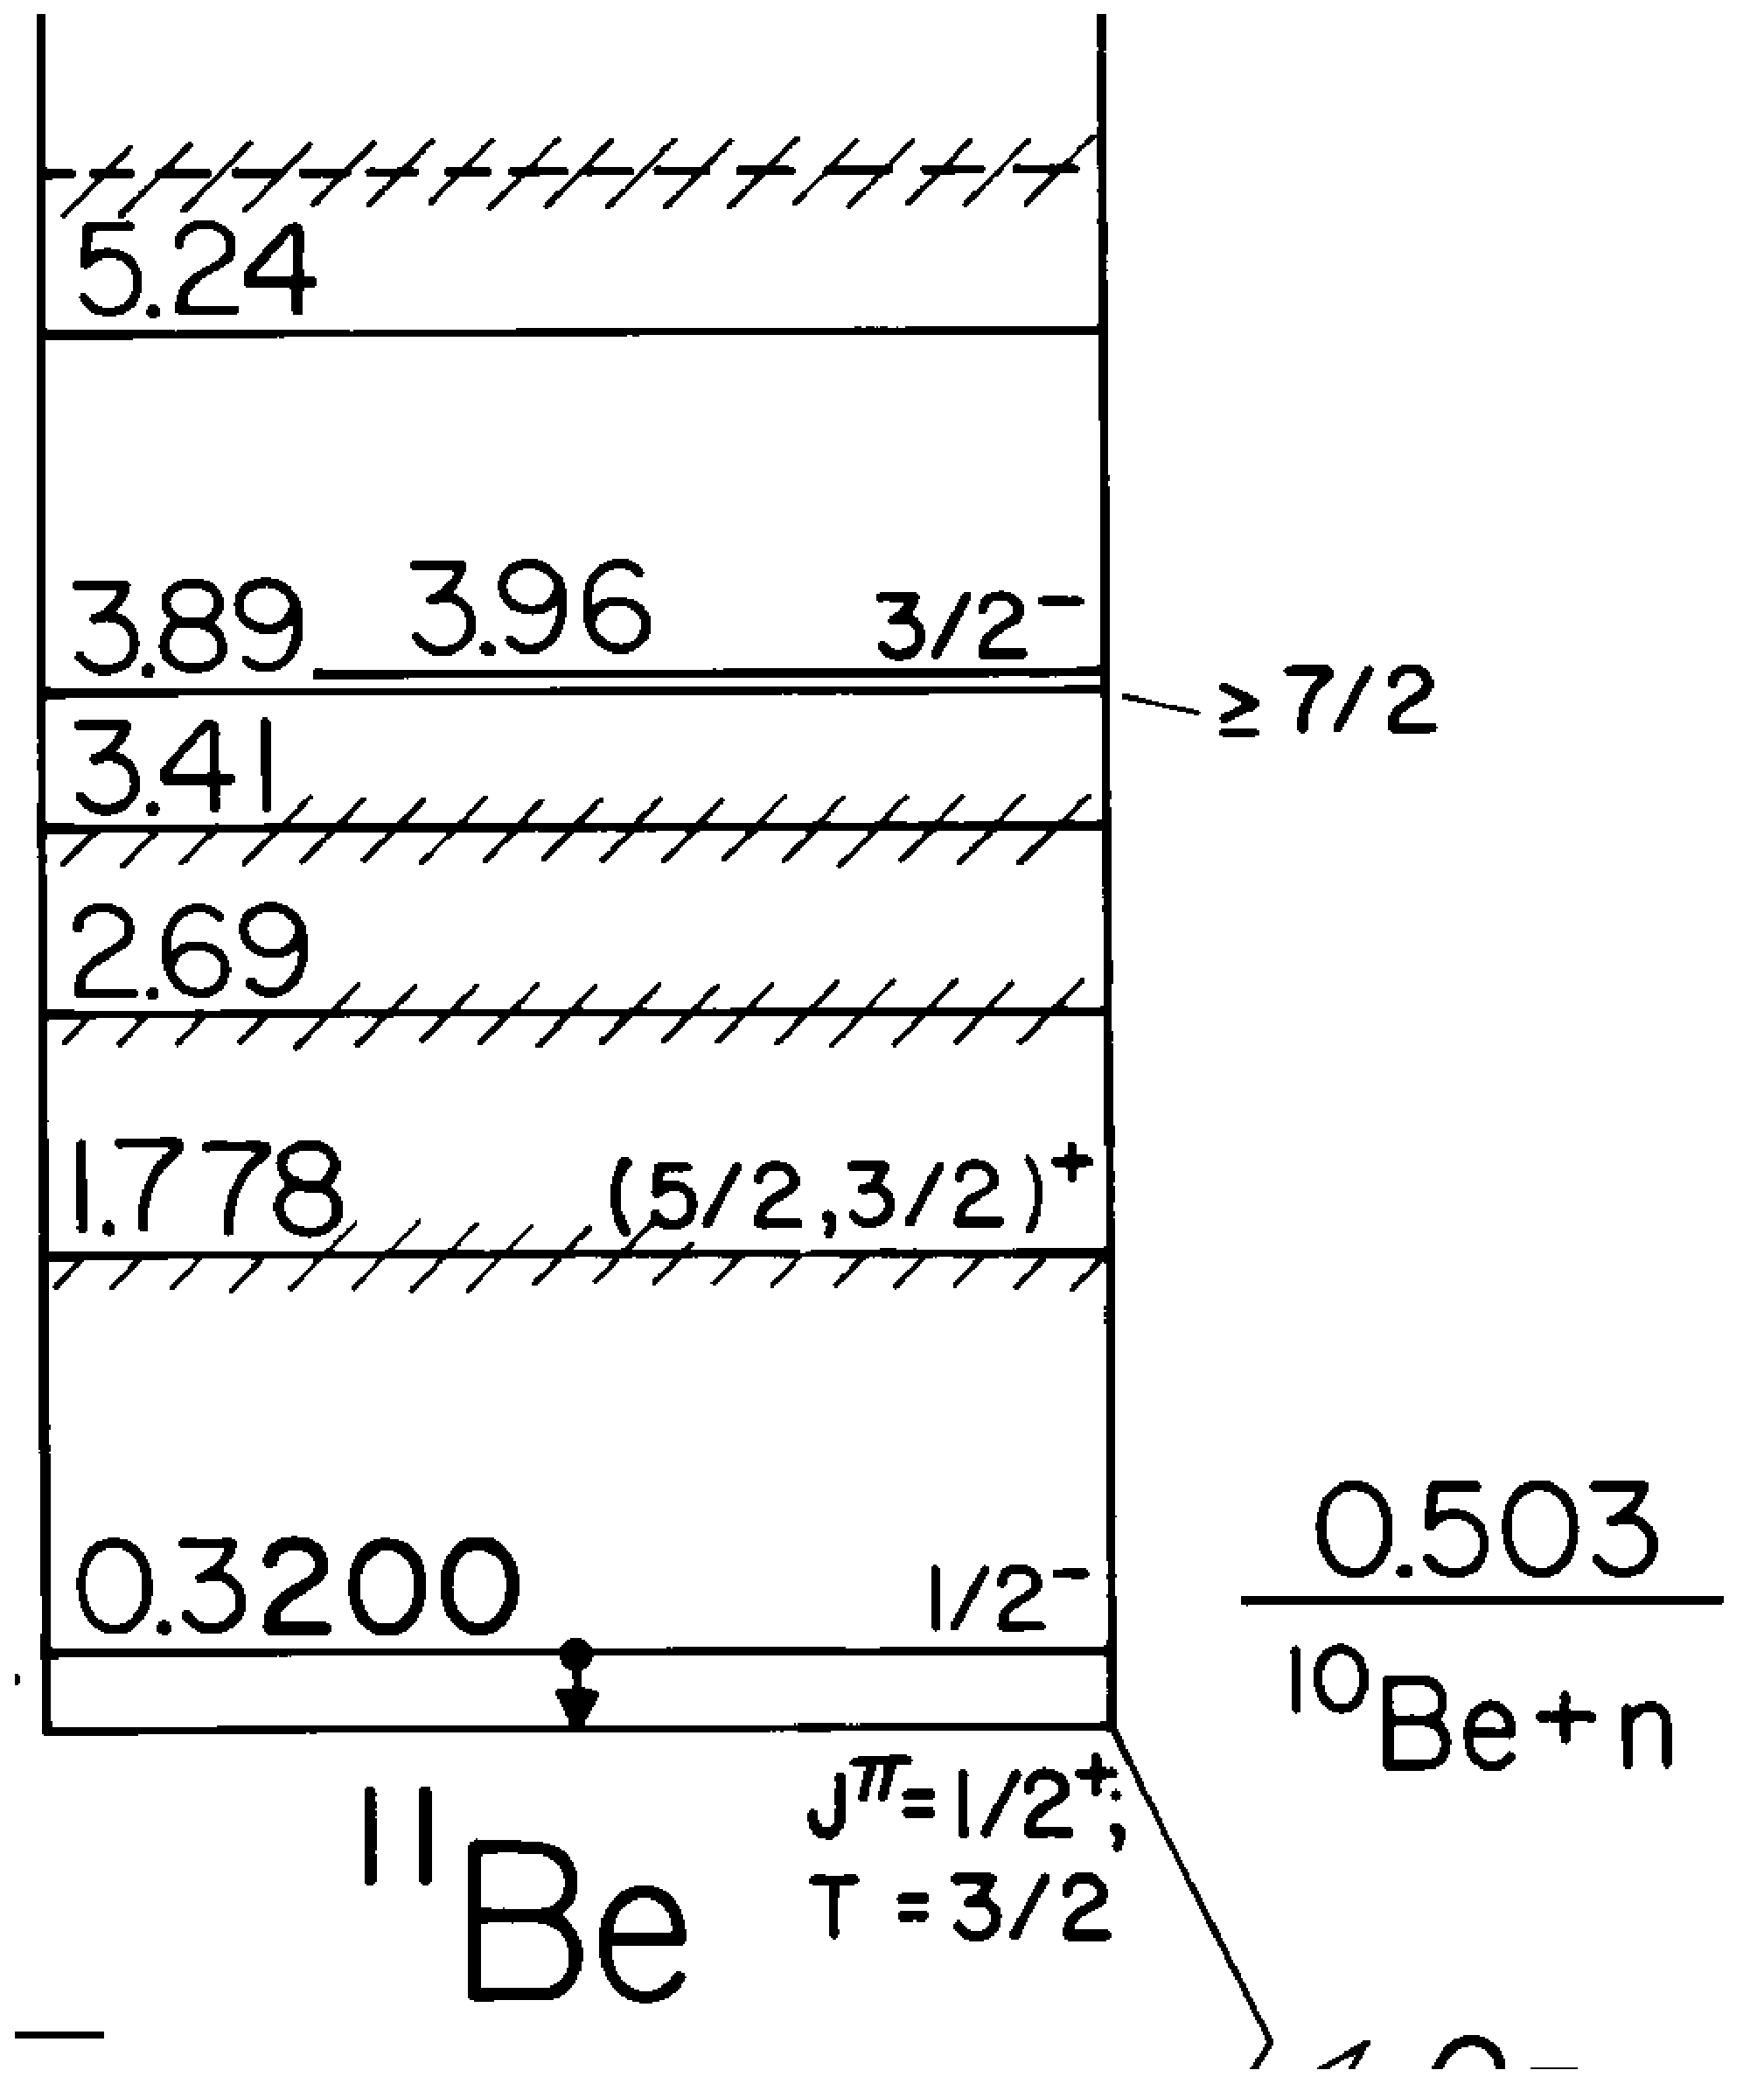
\includegraphics[angle=0,height=0.33\textheight]{\images/be11_spectrum_crop.eps} \end{center}

\bc
\column{0.5\linewidth}
\begin{center}  \psframebox[fillcolor=green!15,linecolor=blue,framearc=0.1,fillstyle=solid]{Ground state ($1/2^+$)} \end{center}
\begin{center} 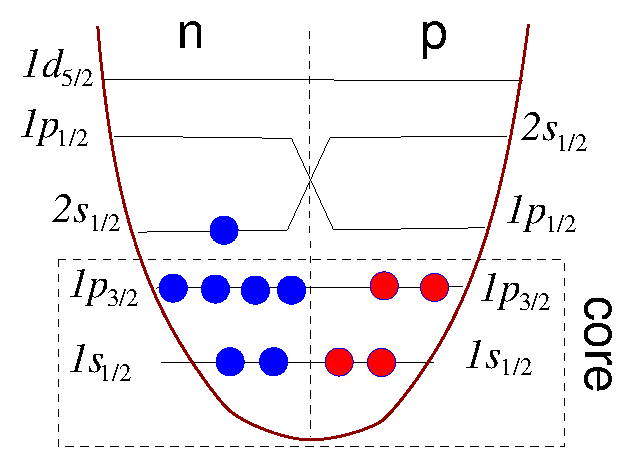
\includegraphics[width=0.45\columnwidth]{\images/be11_capas_inert.eps} \end{center}

\column{0.5\linewidth}
\begin{center} \psframebox[fillcolor=green!15,linecolor=blue,framearc=0.1,fillstyle=solid]{First excited state ($1/2^-$)}  \end{center}
\begin{center} 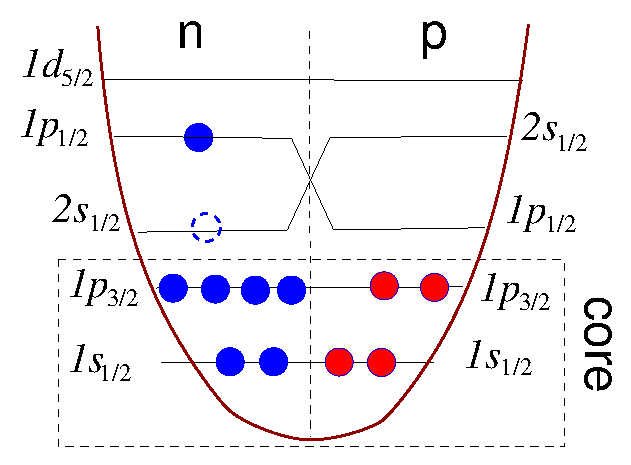
\includegraphics[width=0.45\columnwidth]{\images/be11_capas_j12n.eps} \end{center}
\ec

\end{frame}

%----------------------------------------------------------------------------------------
\slide{Models for inelastic excitations}
{\blue Microscopically}, what we describe in both cases are quantum transitions between discrete or continuum states:

%\vspace{1cm}

\begin{columns}
\column{0.5\textwidth}
\begin{figure}{\par \resizebox*{0.65\textwidth}{!}
{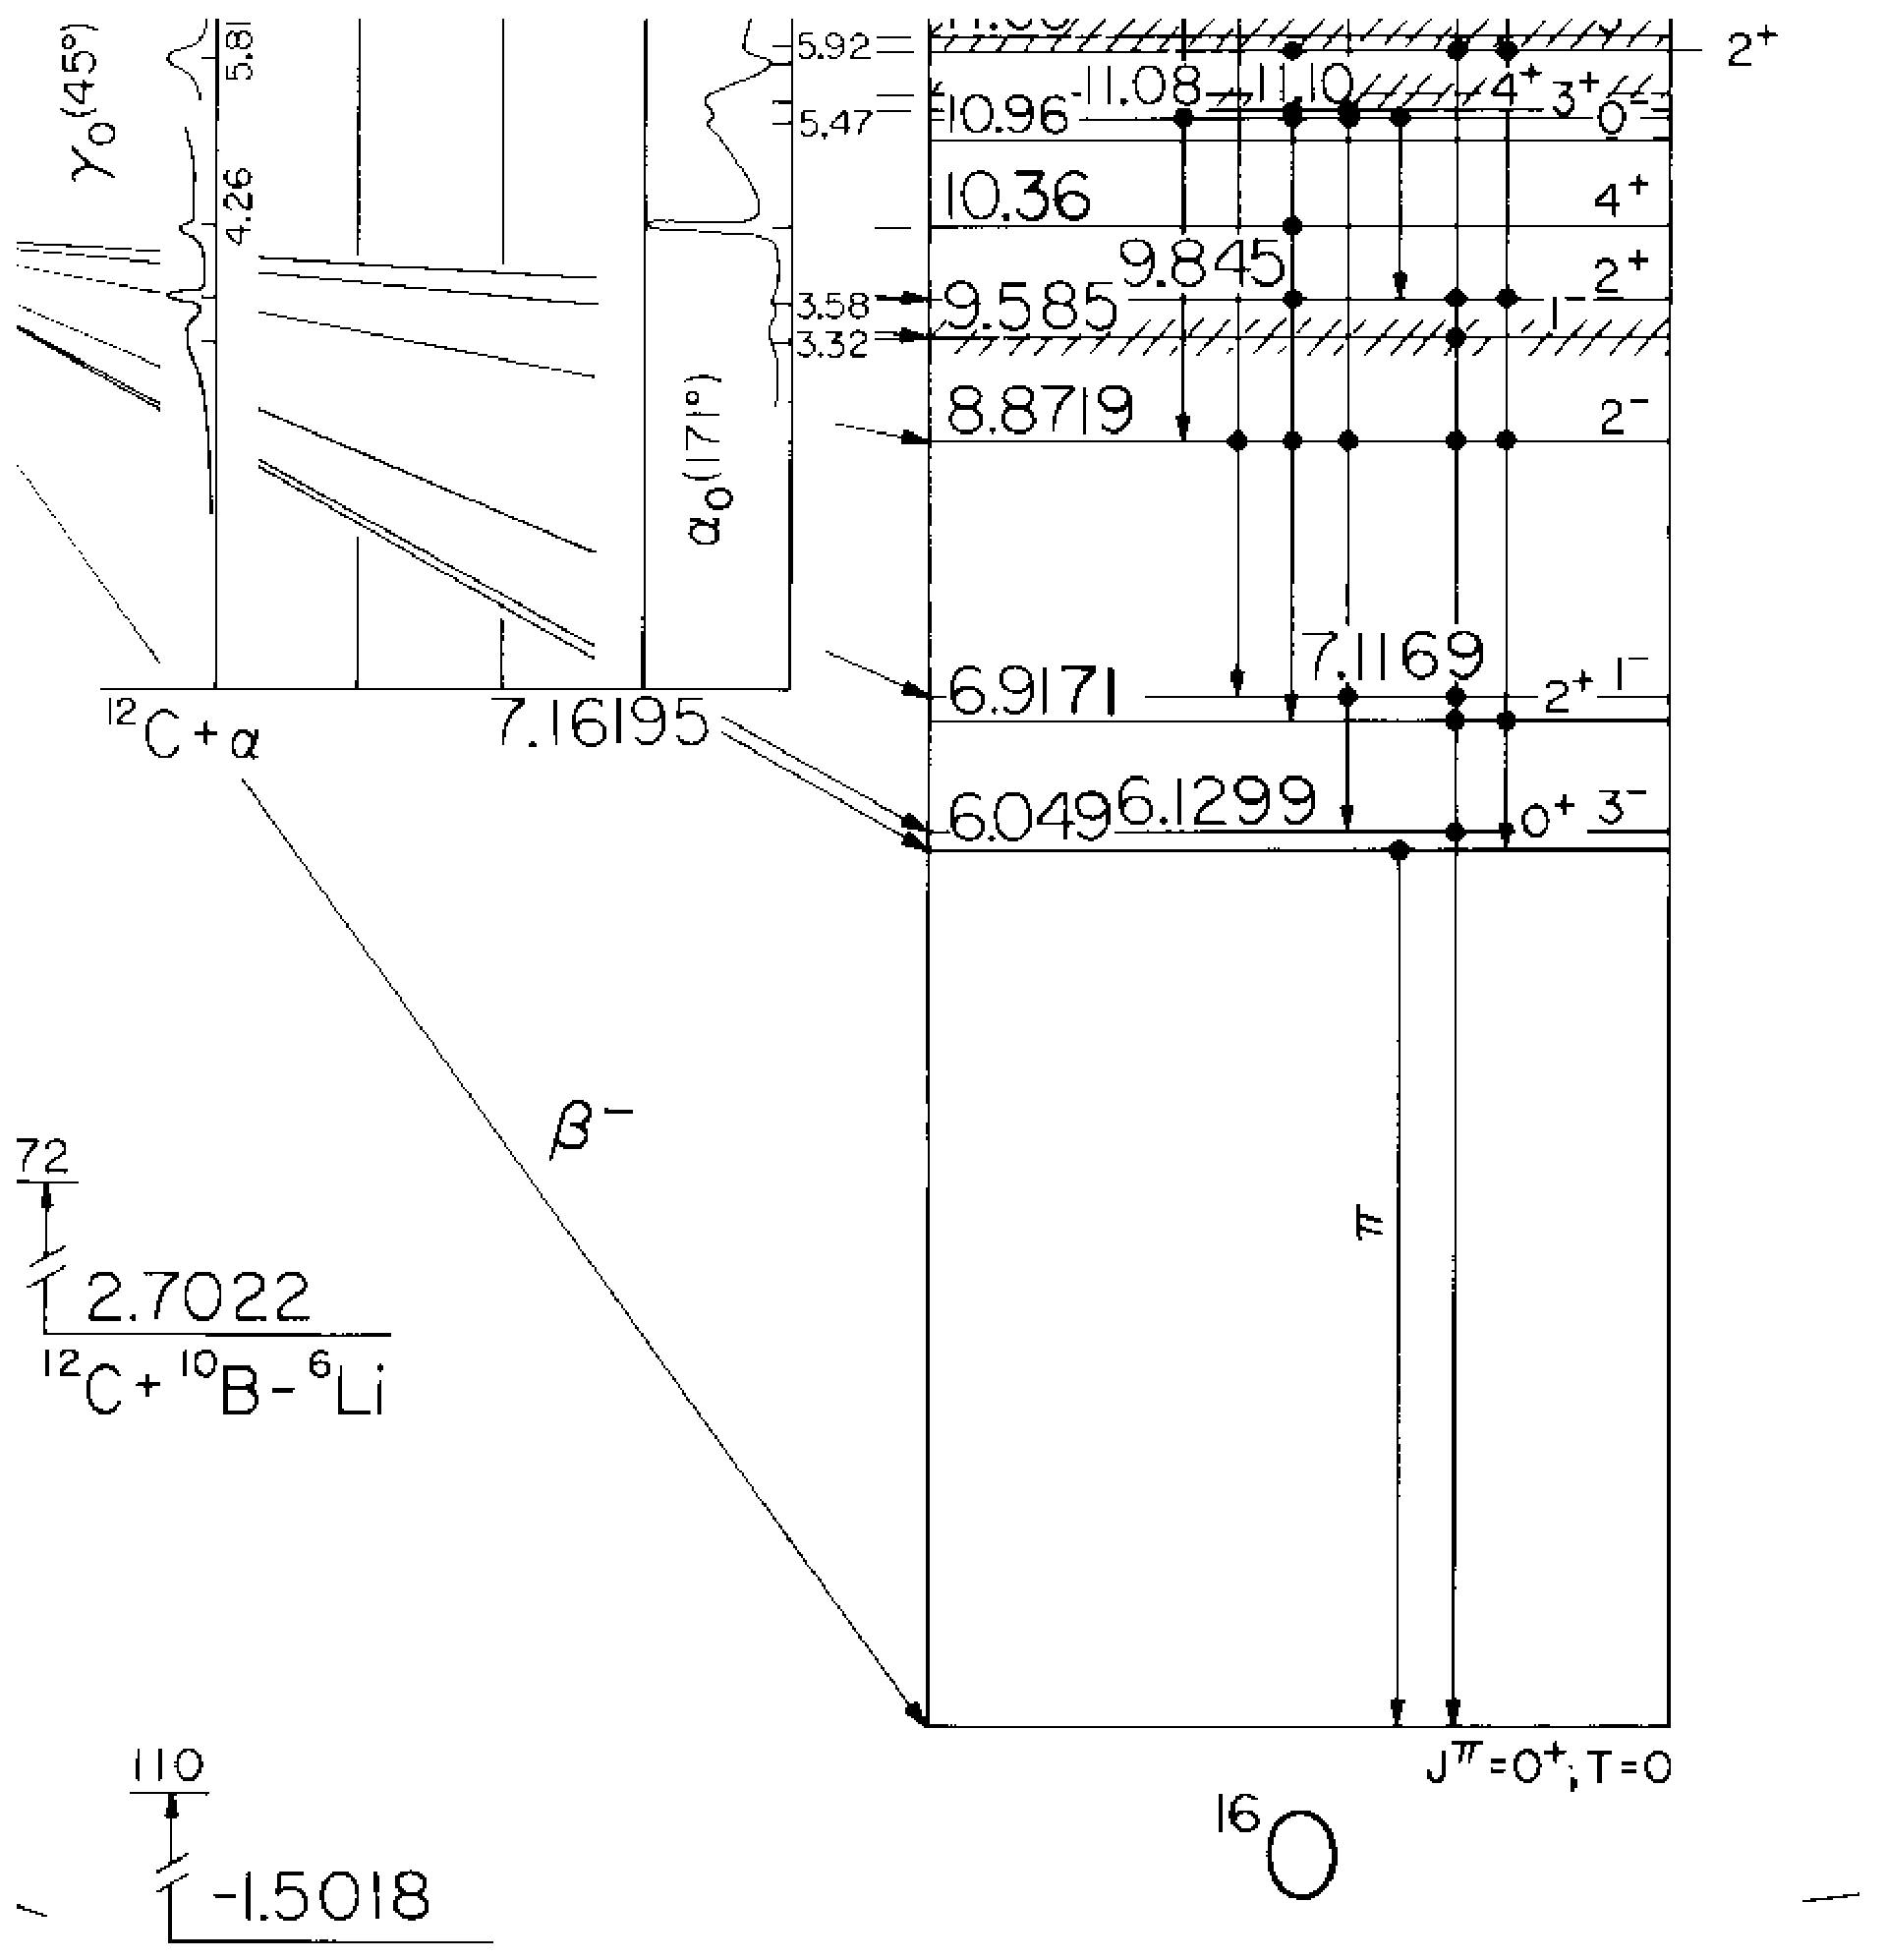
\includegraphics[angle=0]{\images/o16_spectrum.eps}} \par}
\end{figure}
\column{0.5\textwidth}
\begin{figure}{\par \resizebox*{0.5\textwidth}{!}
{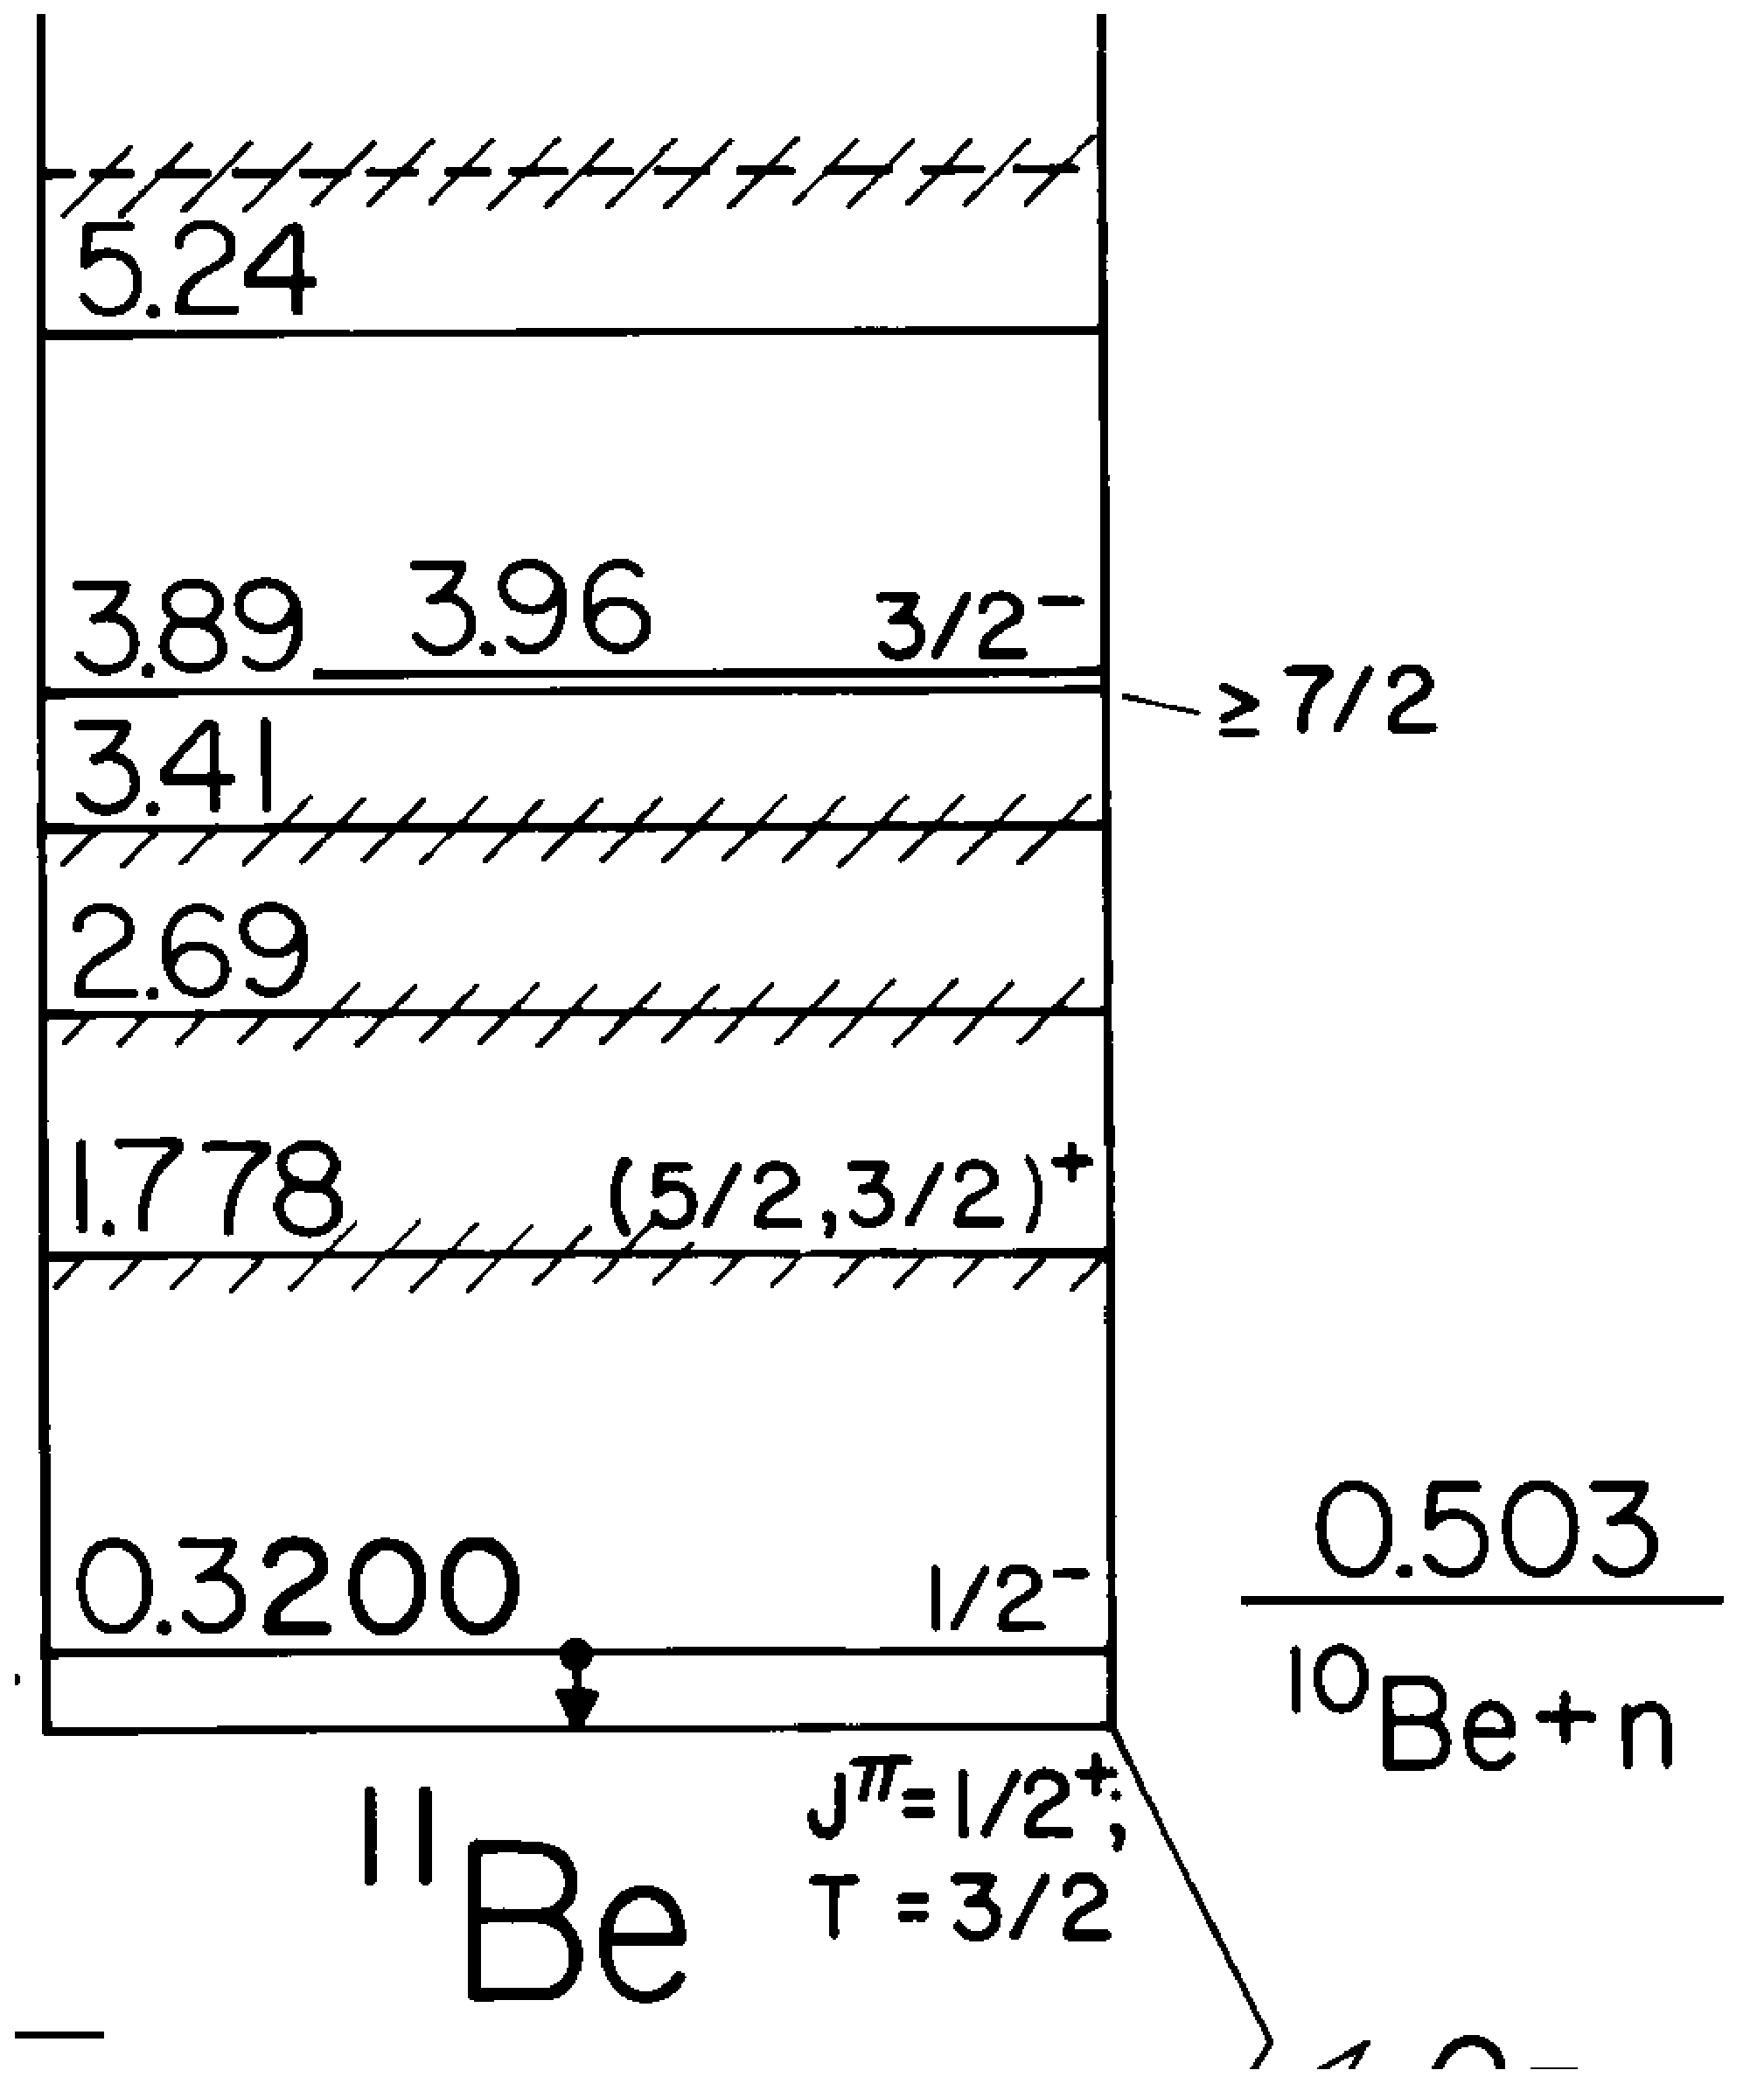
\includegraphics[angle=0]{\images/be11_spectrum_crop.eps}} \par}
\end{figure}
\end{columns}

\vspace{0.5cm}

\ding{43}{\em \magenta Collective excitations can be regarded as a coherent superposition of many single-particle excitations.}
\end{frame}


%-------------------------------------------------------------------------------------------------------
\slide{}
\begin{itemize}
\item By doing inelastic scattering experiments we {\it measure} the {\it response} of the nucleus to an external field (Coulomb, nuclear). This response is related to some structure property of the nucleus. 

\item[] Example: for a {\brick Coulomb} field:

$$ % BM convention 
\psframebox[linecolor=red,framearc=0.1]{
B(E\lambda; i \to f) = \frac{1}{2I_i +1} |\langle \Psi_f | {\cal M}(E \lambda) | \Psi_i \rangle |^2 
}
$$ 
where {\brick ${\cal M}(E\lambda, \mu)$}  is the electric multipole operator:
$$
\psframebox[linecolor=red,framearc=0.1]{
 {\cal M}(E\lambda, \mu) \equiv e \sum_i^{Z_p} r_i^\lambda  Y_{\lambda \mu}^{*}(\hat r_i) 
}%ps
$$


\item The structure $\Psi_{i,f}$ can be described in a collective, few-body or microscopic model. 

% \begin{center}
% $$ 
% \psframebox[fillcolor=green!15,linecolor=blue,framearc=0.1,fillstyle=solid]
%   {\mathrm{Probability} \propto |\langle \Psi(2^+) | \hat{V} | \Psi(gs;0^+) \rangle|^2 }   
% $$ 
% \end{center}

%This process can be treated in different ways:
%\begin{itemize}
%\item {\bf Microscopic}: treat all nucleons of the nucleus being excited 
%\item {\bf Collective}: defining some collective (macroscopic) parameters measuring the strength of these couplings. 
%\item {\bf Few-body}: Grouping some nucleons in clusters corresponding to more compact structures. 
%\end{itemize}

\end{itemize}

\end{frame}


% ----------------------------------------------------------------------------------------------------
\slide{Multi-channel case: the coupled-channels method}
We need to incorporate explicitly in the Hamiltonian the internal structure of the nucleus being excited (eg.~ {\verde target}).
$$ 
\psframebox[linecolor=red,framearc=0.1]{
 H = T_R   +  h(\xi)+ V(\bR, \xi)
}
$$


\begin{itemize}
\gitem{$T_R$}: Kinetic energy for projectile-target relative motion.
\gitem{$\{\xi\}$}: Internal degrees of freedom of the target (depend on the model).
\gitem{$h(\xi)$}: Internal Hamiltonian of the target.
$$
\psframebox[linecolor=red,framearc=0.1]{
h(\xi)\phi_{n}(\xi)  =  \varepsilon_{n}\phi_{n}(\xi)
}
$$

\gitem{$V(\bR, \xi)$}: Projectile-target interaction.
%, eg:
%$$
%V(\bR, \xi) = \sum_{i=1}^{N} V_{pi}(\br_{pi})
%$$

% \pause 
% \item[] {\bf Eg.:} $^7$Li=$\alpha+t$ $\Rightarrow$ {\verde $\{\xi\} \equiv \bf r$}
% $$
% V_\mathrm{p-7Li}({\bf R}, {\bf r})= V_\mathrm{p-t}\left({\bf R} +\frac{4}{7}{\bf r}\right) 
% + 
% V_\mathrm{p-\alpha}\left({\bf R} +\frac{3}{7}{\bf r}\right)
% $$
\end{itemize}
\end{frame}




% ----------------------------------------------------------------------------------------------------
\slide{Defining the modelspace: d+\nuc{10}{Be} $\rightarrow$ d+\nuc{10}{Be*} example}

\begin{center}
\begin{columns}
\column{0.6\textwidth}
\hspace{2cm}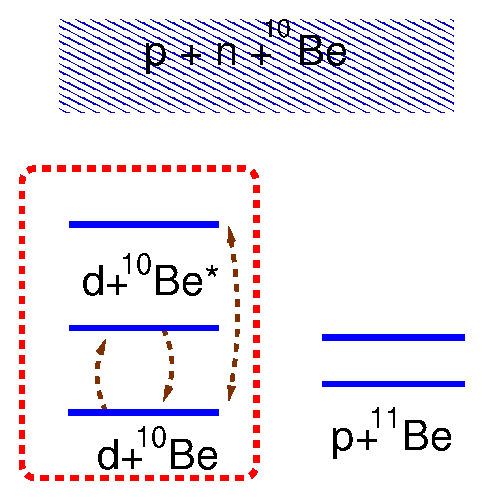
\includegraphics[width=0.4\columnwidth]{\images/be10d_modelspace_ine.eps}
\column{0.4\textwidth}
\psframebox[fillcolor=yellow!25,linecolor=black,fillstyle=solid,framearc=0.1]{
\parbox{0.8\columnwidth}{
 \ding{43} P space composed by ground states (elastic channel) and some excited states (inelastic scattering)  
}%parbox
}%frame
\end{columns}
\end{center}

Boundary conditions:

$$
 \Psi^{(+)}_{\bK_0}(\bR,\xi)   \xrightarrow{R \gg}  \underbrace{\vphantom{\sum_{n>0}} e^{i \bK_0 \cdot \bR} \phi_0(\xi)}_{\mathrm{\blue incident}}   
                          +  \underbrace{\vphantom{\sum_{n>0}} {\red f_{0,0}(\theta)} \frac{e^{i K_0 R}}{R} \phi_0(\xi)}_{\mathrm{\blue elastic}}
                          + \underbrace{\sum_{n>0} {\red f_{n,0}(\theta)}  \frac{e^{i K_n R}}{R}  \phi_n(\xi)}_{\mathrm{\blue inelastic}}
$$

Cross sections:
$$
 \left (  \frac{d\sigma(\theta)}{d\Omega} \right )_{0\rightarrow n} = \frac{K_n}{K_0}  |{\red f_{n,0}(\theta)} |^2 
$$

\end{frame}






% ----------------------------------------------------------------------------------------------------
\slide{CC model wavefunction (target excitation)}

We expand the total wave function in a subset of internal states (the {\cal P} space):
$$
\psframebox[linecolor=red,framearc=0.1]{
\Psi_\mathrm{model}(\bR,\xi)=\phi_{0}(\xi)\chi_{0}(\bK_0,\bR)+ \sum_{n>0} \phi_{n}(\xi)\chi_{n}(\bK_n,\bR)  
}
$$

Boundary conditions for  the $\chi_{n}(\bR)$ (unknowns):

\begin{align*}
\chi_0^{(+)}(\bK_0,\bR) & \rightarrow  e^{i \bK_0 \cdot \bR}  + {\red f_{0,0}(\theta)} \frac{e^{i K_0 R}}{R} 
\quad \quad  \textrm{\blue for n=0 (elastic)} \\
\chi_n^{(+)}(\bK_n,\bR) & \rightarrow                           {\red f_{n,0}(\theta)} \frac{e^{i K_n R}}{R} 
\quad  \quad \quad \quad \textrm{\blue for n>0 (non-elastic)}
\end{align*}

\end{frame}






% ----------------------------------------------------------------------------------------------------
\slide{Calculation of $\chi_n^{(+)}(\bR)$: the coupled equations}

\begin{itemize}
\item The model wavefunction must satisfy the Schr\"odinger equation:
$$
 [H-E]\Psi^{(+)}_\mathrm{model}(\bR,\xi)=0
$$

\item Multiply on the left by each $\phi_{n}(\xi)^*$, and integrate over $\xi$ $\Rightarrow$ coupled channels equations for {\verde $\{\chi_{n}(\bR) \}$:}
%Projecting onto the internal states one gets a system of coupled-equations for the functions 
$$
\psframebox[linecolor=red,framearc=0.1]{
\left[E-\varepsilon_{n}-T_R -V_{n,n}(\bR) \right] \chi_{n}(\bR)  = 
\sum_{n' \neq n} V_{n,n'}(\bR) \chi_{n'}(\bR) 
}%psframebox
$$


\item {\verde Coupling potentials:}
$$
\psframebox[linecolor=red,framearc=0.1,fillcolor=magenta!5,fillstyle=solid]{
V_{n,n'}(\bR) = \int   d \xi \phi_{n'}(\xi)^* V(\bR, \xi) \phi_{n}(\xi) 
}%psframebox
$$

\item[\ding{43}] {\small \em \blue $\phi_{n}(\xi)$ will depend on the assumed structure model 
(collective, few-body, etc).}

\end{itemize}
\end{frame}


% ----------------------------------------------------------------------------------------------------
\slide{Optical Model vs. Coupled-Channels method}

\vspace{-0.5cm}
%\twocolumn[lcolwidth=0.4\linewidth, rcolwidth=0.6\linewidth,frsep=-2pt,colsep=0pt]{
\begin{columns}[t]
\column{0.35\textwidth}
\begin{center}\miframebox{Optical Model}\end{center}
\begin{itemize}
\small
\setlength{\itemsep}{12pt}

\gitem{The Hamiltonian}: \\ $ H = T_R   +   V(\bR)$

\gitem{Internal states}: Just $\phi_0(\xi)$
 
\gitem{Model wavefunction:} \\ $\Psi_\mathrm{mod}(\bR,\xi) \equiv \chi_{0}(\bK,\bR) \phi_0(\xi) $

\gitem {Schr\"odinger equation:} \\ $[H-E]\chi_0(\bK,\bR)=0$
\end{itemize}
\column{0.65\textwidth}
%}{%twocol
\pause 
\begin{center}\miframebox{Coupled-channels method}\end{center}
\begin{itemize}
\small
\setlength{\itemsep}{12pt}

\gitem{The Hamiltonian}: \\ $ H = T_R   +  h(\xi)+ V(\bR, \xi)$

\gitem{Internal states}: \\ $h(\xi)\phi_{n}(\xi)  =  \varepsilon_{n}\phi_{n}(\xi)$
 
\gitem{Model wavefunction:} \\ 
$\Psi_\mathrm{model}(\bR,\xi)=\phi_{0}(\xi)\chi_{0}(\bK,\bR)+ \sum_{n>0} \phi_{n}(\xi)\chi_{n}(\bK,\bR) $

\gitem {Schr\"odinger equation:} 
\begin{center} $[H-E]\Psi_\mathrm{model}(\bR,\xi)=0$ \end{center}
$$\Downarrow$$
$$\left[E-\varepsilon_{n}-T_R -V_{n,n}(\bR) \right] \chi_{n}(\bK,\bR)  = 
\sum_{n' \neq n} V_{n,n'}(\bR) \chi_{n'}(\bK,\bR) $$
\end{itemize}
\end{columns}
%}%twocolumn

\end{frame}








% ----------------------------------------------------------------------------------------------------
\slide{A first-order formula for $f(\theta)$: the DWBA approximation }
\begin{itemize}
\item Assume that we can write the p-t interaction as: $V(\bR,\xi)= V_0(R) + \Delta V(\bR,\xi)$

\item Use central $V_0(R)$ part to calculate the (distorted) waves for p-t relative motion:

\begin{align*}
\left[\hat{T}_{\bR} + V_0(R) - E_i \right] \chi^{(+)}_{i}(\bK_i,\bR)  =  0 \quad \quad (E_i= E - \varepsilon_i) \\ 
\left[ \hat{T}_{\bR} + V_0(R) - E_f\right] \chi^{(+)}_{f}(\bK_f,\bR) = 0 \quad \quad (E_f= E - \varepsilon_f) 
\end{align*}


%\item Apply the two-potential formula taking as auxiliary potential $U_\beta(\bR) \equiv V_0(\bR)$:
%$$ f^\mathrm{exact}_{i \rightarrow f}(\theta)=
% -\frac{\mu}{2 \pi \hbar^2} \int  \chi_{f}^{(-)*}(\bK_f,\bR) \phi_{f}^{*}(\xi) ~\Delta V(\bR,\xi)~ \Psi_{i}^{(+)}(\bK_i,\bR) ~d\xi d\bR
%$$
%with 
%\item Make the {\blue Born approximation}: 
%$\Psi^{(+)}_{\bK_i}(\bR,\xi) \simeq \chi^{(+)}_{i}(\bK_i,\bR) \phi_i(\xi) $, with


\item In first order of $\Delta V(\bR,\xi)$ ({\blue DWBA}) :
$$
\psframebox[fillcolor=magenta!8,linecolor=red,framearc=0.1,fillstyle=solid]{
f^\mathrm{DWBA}_{i \rightarrow f}(\theta)=-\frac{\mu}{2 \pi \hbar^2} \int ~\chi_{f}^{(-)*}(\bK_f,\bR)~ \Delta V_{if} (\bR) ~\chi_{i}^{(+)}(\bK_i,\bR)~ d\bR 
}%psframe
$$
with the {\blue transition potential}:
$$
\psframebox[fillcolor=magenta!8,linecolor=red,framearc=0.1,fillstyle=none]{
\Delta V_{if}(\bR) \equiv  \int \phi_{f}^{*}(\xi) ~ \Delta V(\bR,\xi) ~ \phi_{i}(\xi) ~ d\xi 
}%
$$
\end{itemize}
\end{frame}


%-------------------------------------------------------------------------
\slide{Physical interpretation of the DWBA method}
\begin{itemize}
\item DWBA can be interpreted as a first-order approximation of a full coupled-channels calculation:

\vspace{0.5cm}

\begin{center}
\begin{columns}
\column{0.5\linewidth}
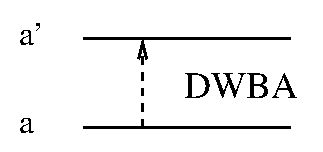
\includegraphics[height=1.5cm]{\images/dwba.eps}
\column{0.5\linewidth}
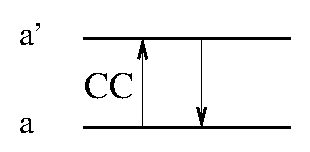
\includegraphics[height=1.5cm]{\images/cc.eps}
\end{columns}
\end{center}

\vspace{0.5cm}

\item The auxiliary potential $U_\beta$ generating the entrance and exit distorted waves is usually chosen in order to reproduce the elastic scattering at the corresponding c.m. energy.

\end{itemize}

\end{frame}


%-----------------------------
\subsection{Models for inelastic scattering}

\slide{}
\begin{center}
\psframebox[fillcolor=green!10,linecolor=blue,framearc=0.1,fillstyle=solid,framesep=5pt]{
Models for inelastic scattering
}%psframe
\end{center} 
\end{frame}



% ----------------------------------------------------------------------------------
\slide{Inelastic scattering in a few-body model}

\begin{itemize}
\gitem{Some nuclei allow a description in terms of two or more clusters:} \\ 
d=p+n,  \nuc{6}{Li}=$\alpha$+d, \nuc{7}{Li}=$\alpha$+\nuc{3}{H}. 

\gitem{Projectile-target interaction:}
 $$ 
 V(\bR,\xi) \equiv V(\bR,\br)= U_{1}(\br_1) + U_2(\br_2)
 $$

%\parbox{0.7\textwidth}{
\psframebox[fillcolor=green!10,linecolor=blue,framearc=0.1,fillstyle=solid]{
\begin{minipage}{.55\textwidth}
%\begin{columns}
%\column{0.3\textwidth}
\textcolor{blue}{Example:} $^7$Li=$\alpha$+t
 $$
 \br_\alpha= \bR - \frac{m_t}{m_\alpha+m_t} \br ;
 \quad 
 \br_t= \bR + \frac{m_\alpha}{m_\alpha+m_t}\br
 $$
{\blue Internal states:} $$[T_\br + V_{\alpha-t}(\br) - \varepsilon_n ]\phi_n(\br)=0$$
\end{minipage}
%\column{0.3\textwidth}
\begin{minipage}{.35\textwidth}
\begin{center}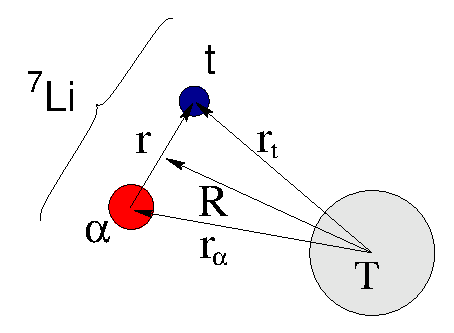
\includegraphics[width=0.7\columnwidth]{\images/li7t_coord.eps}\end{center}
%\end{columns}
\end{minipage}
%}%parbox
}%psframe

\gitem{Transition potentials:}
 $$
\psframebox[linecolor=red,framearc=0.1]{
 V_{n,n'}(\mathbf{R})=\int d\mathbf{r}\phi_{n}^{*}(\br)\left[U_{1}(\br_1) + U_2(\br_2)\right] \phi_{n'}(\br)
}
$$ 

\end{itemize}

\end{frame}



% ----------------------------------------------------------------------------------
\slide{Example: \nuc{7}{Li}($\alpha$+$t$) +\nuc{208}{Pb} at 68 MeV}

%{\bf Example:} \nuc{7}{Li}($\alpha$+$t$) +\nuc{208}{Pb} at 68 MeV {\verde (Phys. Lett. 139B (1984) 150)}: 
%\ding{43}    Uses $\alpha$+t model for \nuc{7}{Li}
%$$
%V_{n,n'}(\bR)=\int d\br \phi_{n}^{*}(\br)
%\left[V_\mathrm{\alpha}(\br_{\alpha}) + V_\mathrm{t}(\br_{t}) \right]
%\phi_{n'}(\br)  ; \quad  n=0,1
%$$

\ding{233} CC calculation with 2 channels (3/2$^-$, 1/2$^-$)  {\verde (Phys. Lett. 139B (1984) 150)}
\begin{columns}
\column{0.4\textwidth}
\begin{center}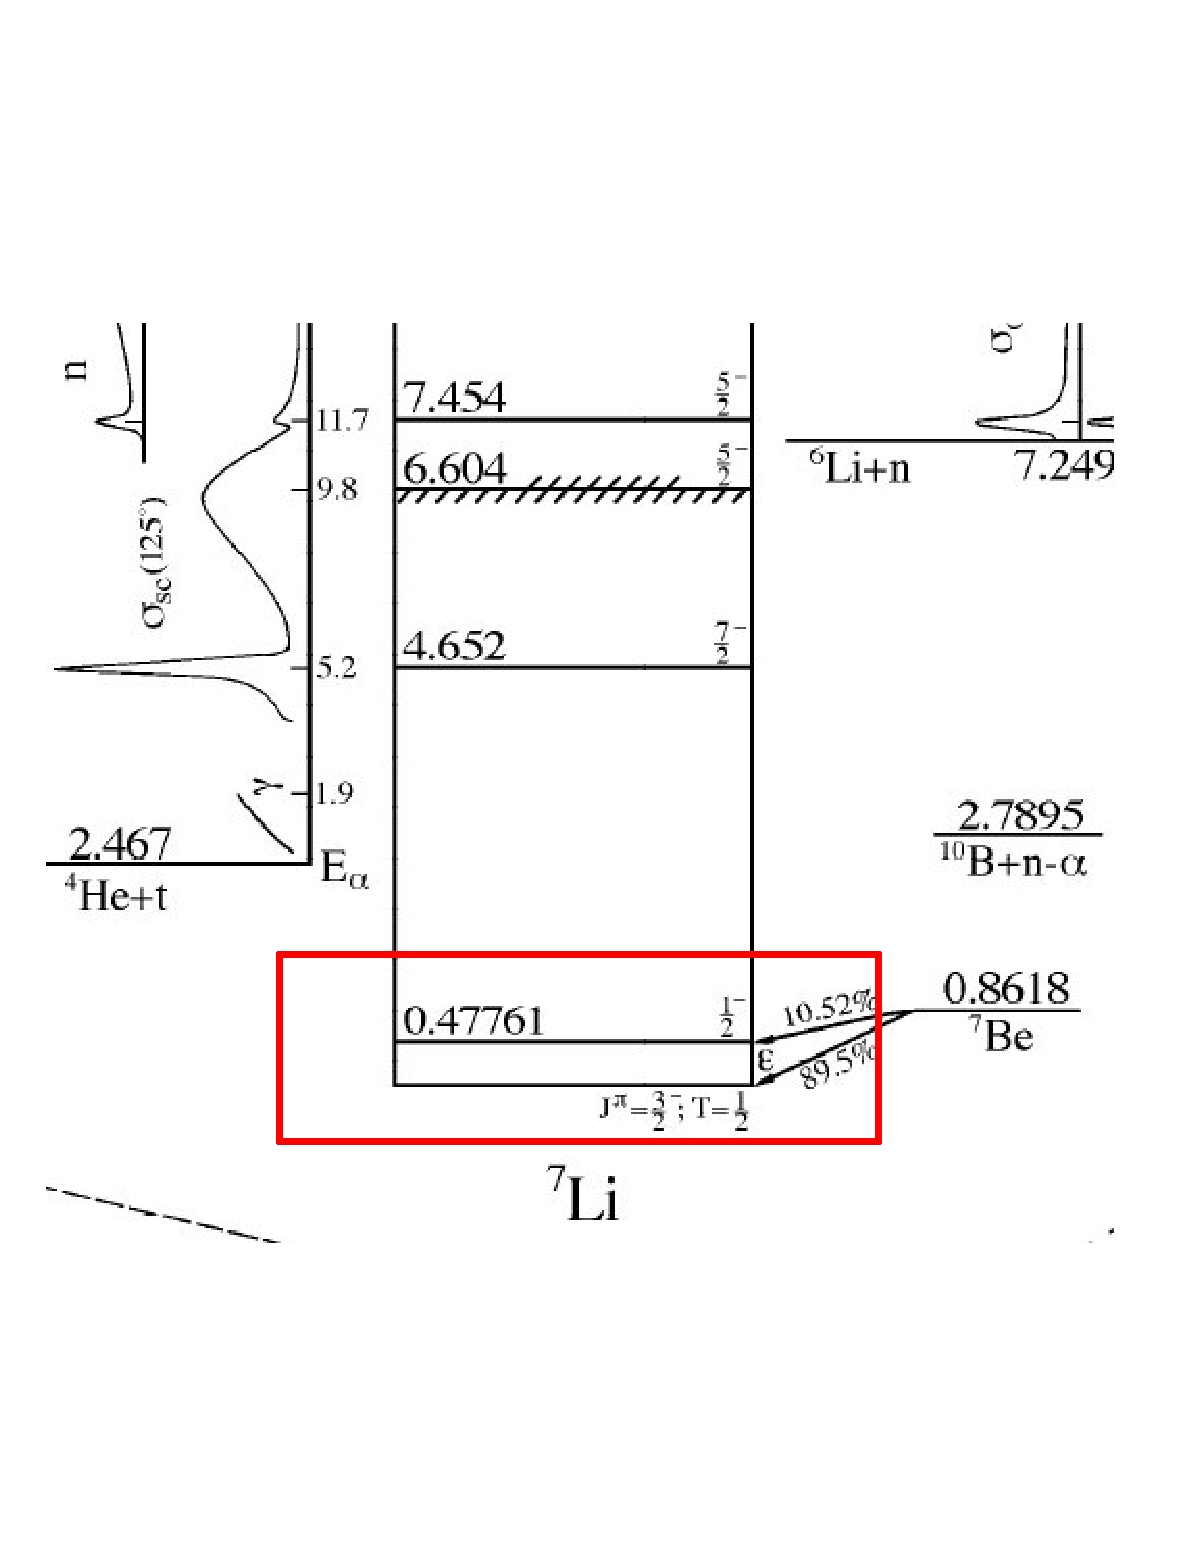
\includegraphics[height=6.0cm]{\images/li7spectrum2.eps} \end{center}
\column{0.5\textwidth}
\begin{center}
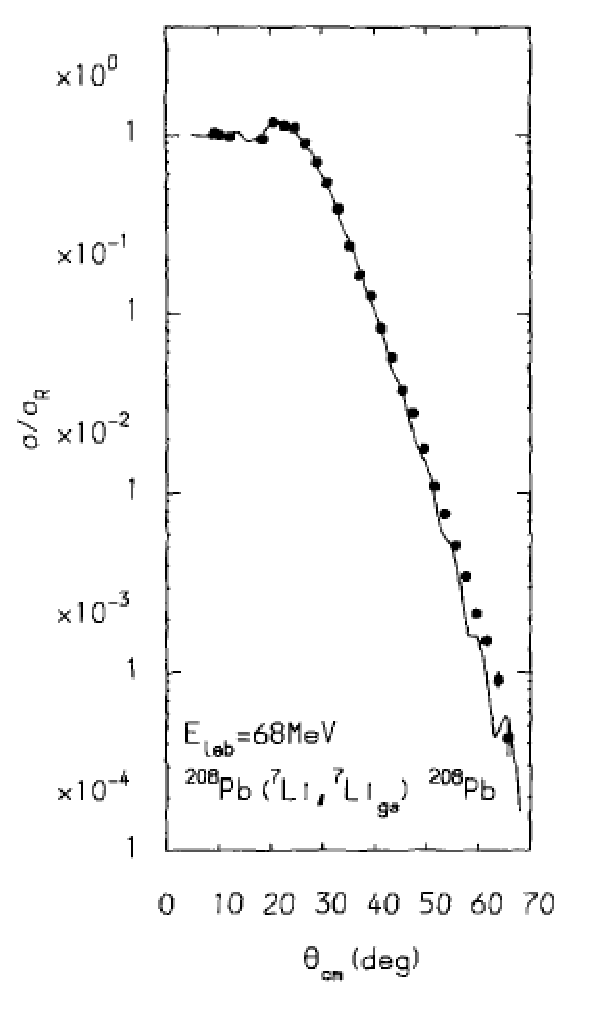
\includegraphics[height=5.5cm]{\images/li7pb_e70_el.eps} 

\includegraphics[height=5.5cm]{\images/li7pb_e70_inel.eps} 
\end{center}
\end{columns}
\end{frame}





